\documentclass[11pt,letterpaper]{article}
\usepackage[margin=0.85in,bottom=0.9in]{geometry}
\usepackage[T1]{fontenc}
\usepackage{newtxtext,newtxmath}
\renewcommand{\ttdefault}{lmtt}
\usepackage{graphicx,booktabs,tabularx,array,enumitem,titlesec,xcolor,caption,float,fancyhdr,microtype}
\usepackage[hidelinks]{hyperref}

\definecolor{ink2}{HTML}{52514E}
\definecolor{pendfill}{HTML}{FFF1C2}
\definecolor{pendline}{HTML}{C98500}
\definecolor{boxfill}{HTML}{F3F2EE}

\setlist{nosep,leftmargin=1.3em}
\setlist[itemize]{label=$\bullet$}
\setlength{\parskip}{4pt}
\setlength{\parindent}{0pt}
\titleformat{\section}{\large\bfseries}{\thesection.}{0.5em}{}
\titleformat{\subsection}{\normalsize\bfseries}{\thesubsection}{0.5em}{}
\titlespacing*{\section}{0pt}{10pt}{2pt}
\titlespacing*{\subsection}{0pt}{7pt}{1pt}
\titlespacing*{\paragraph}{0pt}{4pt}{0.6em}
\captionsetup{font=small,labelfont=bf,skip=4pt}
\renewcommand{\arraystretch}{1.12}
\setcounter{topnumber}{3}\setcounter{bottomnumber}{2}\setcounter{totalnumber}{4}
\renewcommand{\topfraction}{0.88}\renewcommand{\bottomfraction}{0.7}
\renewcommand{\textfraction}{0.08}\renewcommand{\floatpagefraction}{0.8}
\setlength{\textfloatsep}{10pt plus 2pt minus 2pt}\setlength{\intextsep}{8pt plus 2pt minus 2pt}
\newcolumntype{L}{>{\raggedright\arraybackslash}X}

\pagestyle{fancy}
\fancyhf{}
\renewcommand{\headrulewidth}{0pt}
\fancyfoot[L]{\footnotesize\color{ink2}ExeaLM funding report, draft of 27 November 2026}
\fancyfoot[R]{\footnotesize\color{ink2}\thepage}

% A result that is not in yet. Each one names the run that fills it.
\newcommand{\pend}[1]{\fcolorbox{pendline}{pendfill}{\footnotesize\bfseries PENDING: #1}}
\newcommand{\pendbox}[1]{\par\noindent\fcolorbox{pendline}{pendfill}{\parbox{\dimexpr\linewidth-2\fboxsep-2\fboxrule\relax}{\small\textbf{PENDING:} #1}}\par}
\newcommand{\sect}[1]{\S#1}

\begin{document}

%======================================================================== page 1
\thispagestyle{fancy}
{\LARGE\bfseries Funding ExeaLM-9B, an open model for research and code\par}
\vspace{5pt}
{\normalsize Exea Labs funding report, draft of 27 November 2026. Project lead: Avneh Bhatia.\par}
{\normalsize\color{ink2} Exea Labs is a U.S.\ 501(c)(3) nonprofit research lab run by high school students.\par}
\vspace{4pt}\hrule\vspace{2pt}

\paragraph{The claim.}
A model for research and code has to read long papers and large codebases, and it needs more facts than its weights can hold.
ExeaLM is built for both.
It reads a long document as a \emph{stream}, meaning in windows of 512 tokens (word pieces), carrying what it computed for each window into the next.
Before it answers, it searches a \emph{library} of reference entries and real passages and reads the best match.
We ask for the compute to train ExeaLM at 9 billion parameters (9B), the learned numbers in a model, on one trillion (1T) tokens.
We plan to release the model openly with its library.
The aim is the best open-weight 9B system for research and code, where open-weight means anyone can download and run the trained model.

\paragraph{The evidence.}
A National AI Research Resource (NAIRR) Pilot award gave us 2,000 hours of NVIDIA H100 GPUs (GPU-hours) at the San Diego Supercomputer Center.
With it we trained ExeaLM and our implementation of the design of Alibaba's Qwen3.5 models, the \emph{Qwen3.5-style model}, at equal size, data and tokens.
Each model is scored in \emph{bits per byte}, the information it needs to predict each byte of text it never trained on.
Lower is better.
ExeaLM scored lower than the Qwen3.5-style model on all 18 held-out text sets with each of 3 seeds (independent runs), at both 0.1B and 0.25B parameters.
Its lead was 2.8\% at 0.1B and 1.1\% at 0.25B.
Most of the lead comes from published changes to attention and from ExeaLM's last 20\% of training, which reads streams.
The one new layer type in ExeaLM adds about 0.1\% on text, and it carries exact facts across windows: it finds a pass key placed one window back 28\% of the time, against 9\% for the same model with attention in its place (0.25B, 3 seeds).
On long-context tasks scored as exact match, ExeaLM recalls 12\% to 14\% more text from far back than the Qwen3.5-style model at every size, and the lead does not shrink with size.

\vspace{4pt}
\noindent\colorbox{boxfill}{\begin{minipage}{\dimexpr\linewidth-2\fboxsep\relax}
\vspace{5pt}
\begin{tabularx}{\linewidth}{@{\hspace{4pt}}>{\raggedright\arraybackslash}p{0.29\linewidth}@{\hspace{10pt}}>{\raggedright\arraybackslash}p{0.29\linewidth}@{\hspace{10pt}}L@{}}
{\huge\bfseries +12\%} & {\huge\bfseries 64\%} & {\huge\bfseries 75,000} \\[2pt]
\small more exact recalls of text last seen over 512 tokens back than the Qwen3.5-style model, at 0.1B, 0.25B and 0.5B alike (14\%, 12\%, 12\%; p below $10^{-40}$ at each size). On a pass key in the same window: 0.86 against 0.19 at 0.5B.
&
\small fewer bits per byte on held-out research questions when the 0.1B ExeaLM searches its library (1.645 to 0.590, 3 seeds). The released Qwen3.5-9B-Base scores 1.031 with no library and 0.313 with the same library.
&
\small H100 GPU-hours to pretrain the 9B on 1T tokens, at the speed we measured for the 9B on one node of four H100s. That is \$202,000 to \$299,000 at public on-demand list prices of \$2.69 to \$3.99 per GPU-hour.
\end{tabularx}
\vspace{3pt}
\end{minipage}}
\vspace{2pt}

\paragraph{The ask.}
Tier~1 is about 112,000 H100 GPU-hours, or \$301,000 to \$447,000 at the same prices.
It pays for pretraining, post-training for research and code, evaluation and a 30\% reserve for restarts and data loading.
Tier~2 adds a year of the library's search service on one GPU and support for the team.
We plan to release the weights, the code, the data and the library, each under its sources' licenses.

\paragraph{What is not shown yet.}
Our largest finished models have 0.5B parameters, and the 3B pair is due to finish on the evening of 29 November 2026.
On windows read alone, ExeaLM's lead shrinks with size, from 2.8\% at 0.1B to 0.6\% at 0.5B, and with training length, to 0.6\% at 0.1B trained for 110 tokens per parameter (2 seeds). On long documents read as a stream it is 3.6\% to 5.3\% at every size and length tested.
The library results are from 0.1B models only.
No model we trained finds a pass key two or more windows back: exact retrieval from far back is not solved at these sizes.
With no library, the released Qwen3.5-9B-Base is far ahead of our 0.25B model (0.674 against 1.011 bits per byte, seed 0).
So the 9B claim is for the model with its library, and every benchmark will be reported with and without the library.

\paragraph{Where to check.}
The code and results are at \url{https://github.com/exea-labs/ExeaLM/tree/nairr}.
The trained models and data are at \url{https://huggingface.co/exea-labs}.
Appendix~A gives the file behind each number.

\newpage
%======================================================================== 1
\section{The thesis}

Research and code questions have two features that size alone handles poorly.
The inputs are long.
A research paper runs 4,000 to 10,000 tokens, and code that spans a repository 8,000 to 32,000.
The answers also depend on more facts than weights can hold.
Plain weights store about 2 bits of knowledge per parameter (Allen-Zhu and Li, \emph{Physics of Language Models}, part 3.3).

ExeaLM meets each feature with a part that does not grow with the model.
For long inputs it reads streams.
Each 512-token window is read with the attention keys and values of the window before and the state of its middle layer carried in.
Exact attention therefore reaches one window back, and older text reaches the model through the carried state.
For facts it reads a library.
A keyword search picks the best entry for the question and places it before the question, a method called retrieval-augmented generation (RAG).
Library v2 will add the best real passage as well.

The model is mostly a standard transformer.
Every layer but one is attention with four published changes: an output gate, normalized queries and keys (QK-norm), value residual (ResFormer) and exclusive self-attention (XSA).
The middle layer is a \emph{TONN layer}, the lab's own layer type, a row of small circuits such as convolutions, running sums and state-space memories.

The thesis is that a small model can match much larger models on research and code.
It needs two things: to read long documents as streams, and to search a large library partly written by a larger model.
The evidence so far tests the streams at 0.1B to 0.5B and the library at 0.1B.
It does not yet show the whole at 9B.
At 9B the comparison is direct, because many open models are released near that size, from Qwen3.5-9B and GLM-4-9B to OLMo 3 7B and Seed-Coder-8B.

``Best open 9B for research and code'' will mean two statements on a benchmark suite frozen before the 9B is scored.
System to system, ExeaLM-9B with its library scores at least as well as each compared model given the same library and search.
Model to model, with no library, the scores are reported in full, whatever they show.
The candidate suite covers code (HumanEval+, MBPP+, LiveCodeBench, BigCodeBench, DS-1000), science (GPQA Diamond, SciCode), paper reading (QASPER) and math.
Whether the headline says ``best open 9B'' or ``best fully open 9B'' (open weights, data and code) is still an open decision in the post-training plan.

%======================================================================== 2
\section{Evidence so far}

\subsection{How the models were compared}

All runs in this section are from the NAIRR study on the Expanse cluster. Its results page is \texttt{results/}\allowbreak\texttt{expanse/README.md}, cited below as \sect{N}.
The Qwen3.5-style model has Gated DeltaNet layers, a recurrent layer type, in three of every four layers and gated attention with QK-norm in the fourth.
It is our implementation, trained on our data, and not Alibaba's model.
A plain Llama, the standard transformer, runs beside them up to 0.5B.

ExeaLM and the Qwen3.5-style model have the same size within 1\%.
Every model gets the same data, tokenizer and number of training tokens.
The data is \texttt{slice-30b-r2} of our public pretraining set, 28.5B tokens of which 7.3B are research code.
Each model gets its own learning rate from short checks, and the same schedule.
The last 10\% of steps uses the \emph{anneal mix}, which weights the best sources up.
ExeaLM differs in one recipe step.
Its last 20\% of training reads streams of four windows (its \emph{stream phase}), while the baselines read every window alone.
Scores are bits per byte on 512 fixed windows from each of 18 held-out sets, covering research Python, code, papers, math, web text and Japanese.

\subsection{ExeaLM leads at every finished size}

Table~\ref{tab:main} shows ExeaLM ahead of the Qwen3.5-style model at 0.1B, 0.25B and 0.5B.
At 0.1B and 0.25B, with 3 seeds each, it is ahead on all 54 set-and-seed pairs. The margins are 0.024 to 0.061 bits per byte at 0.1B and 0.007 to 0.026 at 0.25B.
It is also ahead of the plain Llama on all 54 pairs at both sizes.
At 0.5B, with 2 seeds, it is ahead on all 36 set-and-seed pairs, by 0.6\% on windows read alone and 3.6\% on long documents, and ahead of the plain Llama on all 36.

\begin{table}[!htb]
\centering\small
\caption{Bits per byte on held-out text at equal data and tokens (lower is better). ``Windows alone'' reads each 512-token window by itself, mean of 18 sets. ``Long documents'' reads the first 4,096 tokens of each long held-out document as a stream of 8 windows (mean of windows 1 to 7). ExeaLM is ahead in every row. Leads are computed before rounding.}
\label{tab:main}
\setlength{\tabcolsep}{3.6pt}\footnotesize
\begin{tabularx}{\linewidth}{@{}l c ccc c cc c X@{}}
\toprule
& & \multicolumn{4}{c}{Windows alone} & \multicolumn{3}{c}{Long documents} & \\
\cmidrule(lr){3-6}\cmidrule(lr){7-9}
Size & Seeds & ExeaLM & Qwen3.5-style & Llama & Lead & ExeaLM & Qwen3.5-style & Lead & Source \\
\midrule
0.1B & 3 & \textbf{1.157} & 1.190 & 1.200 & 0.034 & \textbf{1.096} & 1.157 & 0.061 & \sect{9}, \sect{10} \\
0.25B & 3 & \textbf{1.014} & 1.026 & 1.041 & 0.011 & \textbf{0.955} & 0.997 & 0.042 & \sect{13}, \sect{15} \\
0.5B & 2 & \textbf{0.933} & 0.939 & 0.958 & 0.005 & \textbf{0.873} & 0.906 & 0.033 & \sect{20} \\
3B, step 14,500$^{*}$ & 1 & \textbf{0.806} & 0.813 & not trained & 0.007 & \multicolumn{3}{c}{after training} & \sect{23} \\
3B, final & 1 & \multicolumn{8}{l}{\pend{3B final, both readings, from the 3B pair due on the evening of 29 November 2026}} \\
\bottomrule
\end{tabularx}
\par\smallskip\raggedright\footnotesize $^{*}$In-run check during training, step 14,500 of 45,688: fixed held-out windows read alone, before the stream phase and the anneal. A different reading from the 18-set mean of the other rows.
\end{table}

The \emph{in-run check} scores a model on 512 fixed held-out windows while it trains.
At 0.5B the in-run lead fell from 0.011 at step 6,000 of 7,825 to 0.004 at the end, mostly in the stream phase (\sect{20}).
At 3B the in-run lead has narrowed from 0.034 at step 3,000 to 0.016 at step 7,500 and 0.007 at step 14,500 (\sect{23}), about 0.001 every 1,000 steps: at that rate the two are about even on windows alone before the stream phase. The long-document reading, where the lead held at every finished size, is read on the finished models.
The 3B ExeaLM switches to the mixed stream phase of Section~3 before its own stream phase, which costs less on windows alone.

The control that a reviewer asks for first is ExeaLM with attention in place of its TONN layer, trained the same way.
At 4.1 tokens per parameter ExeaLM is ahead of it by about 0.1\% at 0.1B and at 0.25B (3 seeds each): at 0.25B by 1.0141 against 1.0154 on windows alone, in all 3 seeds, and by 0.9545 against 0.9556 on long documents (\sect{19}).
So the lead in Table~\ref{tab:main} belongs to the attention changes and the streams, which the Qwen3.5-style model does not have.
Trained longer, the control is ahead. At 110 tokens per parameter, the 9B's ratio, it beats ExeaLM on every reading: 0.958 against 0.960 on windows alone and 0.898 against 0.902 on long documents, on all 18 sets (one seed each, \sect{24}).
Both are far ahead of the Qwen3.5-style model on long documents (0.944), so the recipe's lead holds.
This control measures the TONN layer only as a plain text layer, with the memory circuits off.
The 9B keeps its TONN layer: the library search, the board and the weight edits are TONN circuits, which an attention layer cannot hold, and they are what the TONN layer is for.

\paragraph{Learning per token.}
A second measure counts how many more training steps the Qwen3.5-style model needs to match ExeaLM's in-run score.
The long 0.1B pair trains on 10.4B tokens, about 110 per parameter, close to the 9B run's 108, with two seeds of each model (\sect{24}).
Through step 20,000 of 39,735 the multiplier rose in both seeds, from 1.18 and 1.21 at step 5,000 to 1.34 and 1.41 at step 20,000.
Later matches fall inside the Qwen3.5-style model's own learning-rate decay, where the measure no longer compares like with like.
At the end, neither finished Qwen3.5-style run reaches ExeaLM's final score.

Finished, ExeaLM is ahead in both seeds on every reading: 0.958 against 0.963 bits per byte on windows alone (0.6\%), and 0.902 against 0.946 on long documents read as a stream (4.7\%).
Training 27 times longer shrinks the lead on windows alone at 0.1B, from 0.034 to 0.006, as size does.
The long-document lead shrinks less, from 0.061 to 0.044.
Seed 0 kept the old stream phase, and its in-run lead fell from 0.009 to 0.001 within 1,500 steps of the switch at step 31,788.
Seed 1 switched to the mixed stream phase before its own began and kept 0.006 to 0.008 through the decay; on windows alone it ends 0.008 ahead, against 0.003 for seed 0.

A 0.5B run at 20 tokens per parameter (ExeaLM, its attention-only control and the Qwen3.5-style model; 10B tokens each, one seed) started on 27 November. It tests whether these trends hold at a larger size.

\paragraph{Benchmarks at 0.5B.}
On 7 zero-shot benchmarks (no worked examples in the prompt), ExeaLM's mean accuracy is 0.429 against 0.421 for the Qwen3.5-style model and 0.417 for the plain Llama (2 seeds, \sect{20}).
It is ahead in both seeds and on 5 of 7 tasks, most on SciQ (0.032) and LAMBADA (0.020), which asks for the last word of a passage.
The gaps are small: at 2B training tokens all three models are near chance on two of the tasks.

\subsection{Long documents}

Research and code inputs are longer than one window, so the long-document reading matters most for the 9B.
Read as a stream, ExeaLM's lead on 4,096-token documents is 5.3\% at 0.1B and 4.2\% at 0.25B.
Both have 3 seeds and 54 of 54 pairs ahead (\sect{10}, \sect{15}).
At 0.5B the lead is 3.6\% (2 seeds, \sect{20}).

ExeaLM trained on streams in its last 20\% and the Qwen3.5-style model did not, and any model could use that recipe.
The control is ExeaLM trained without its stream phase.
At 0.1B it is still ahead on all 54 pairs, at 1.132 against 1.157 bits per byte (2.2\%, 3 seeds, \sect{10}).

Figure~\ref{fig:position} follows the lead through documents of 16,384 tokens, read as 32 windows.
That is 8 times the length of the streams ExeaLM read in training.
Over windows 1 to 31 the lead is 5.4\% at 0.1B (1.0726 against 1.1339, 3 seeds) and 4.9\% at 0.25B (0.9471 against 0.9956, one seed, \sect{19}).
At 0.25B it grows along the document, from 0.043 bits per byte in windows 1 to 7 to 0.048 in windows 24 to 31.

\begin{figure}[!htb]
\centering
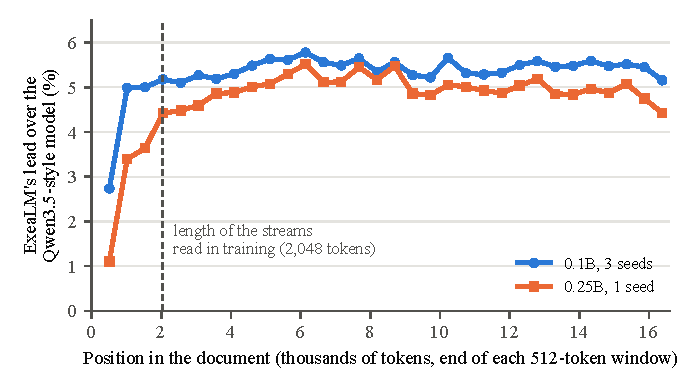
\includegraphics[width=0.68\linewidth]{figs/lead_by_position.pdf}
\caption{ExeaLM's lead over the Qwen3.5-style model for each 512-token window of held-out documents 16,384 tokens long, as a percentage of the Qwen3.5-style model's bits per byte (\sect{19}). Fifteen of the 18 sets have such documents. The lead is smallest in the first window, which has nothing before it, and stays near 5\% to the end of the document.}
\label{fig:position}
\end{figure}

\subsection{Long-context tasks}

Bits per byte is a proxy. The tasks a research or code assistant does are exact: complete the next line of a file, recall a name or number from earlier in a paper, retrieve a fact placed far back.
We scored every finished model on three such tasks over the first 4,096 tokens of held-out documents, read as a stream of 512-token windows (\sect{26}).
Recall asks for a 4-token run whose earlier occurrence is more than a window back; code next line asks for a line that uses an identifier last seen more than a window back (RepoBench's next-line task within one file); the pass key is a 5-digit number placed in Wikipedia text and asked for at the end.
A target counts only if the model's top token is right at every position.

\begin{table}[!htb]
\centering\small
\begin{tabular}{@{}llcccc@{}}
\toprule
Size & Model & Recall & Code next line & Pass key, same window & One window back \\
\midrule
0.1B$^{*}$ & ExeaLM & 0.268 & 0.042 & \textbf{0.648} & \textbf{0.078} \\
 & Qwen3.5-style & 0.235 & 0.038 & 0.047 & 0.000 \\
0.25B & ExeaLM & 0.241 & 0.035 & \textbf{0.766} & \textbf{0.281} \\
 & Attention in place of TONN & 0.243 & 0.035 & 0.635 & 0.094 \\
 & Qwen3.5-style & 0.215 & 0.032 & 0.016 & 0.000 \\
0.5B & ExeaLM & \textbf{0.282} & \textbf{0.045} & \textbf{0.859} & \textbf{0.266} \\
 & Qwen3.5-style & 0.252 & 0.042 & 0.188 & 0.000 \\
\bottomrule
\end{tabular}
\par\smallskip\raggedright\footnotesize Exact-match rate, mean over seeds (0.1B and 0.5B: 2 seeds; 0.25B: 3). $^{*}$The 0.1B pair trained to 111 tokens per parameter. Every target is scored by both models, and the differences are tested target by target (\sect{26}).
\caption{Long-context tasks as exact match.}
\label{tab:longctx}
\end{table}

Against the Qwen3.5-style model ExeaLM is ahead on every task at every size: 12\% to 14\% more recalls (p below $10^{-40}$ at each size), 7\% to 10\% more code lines (p at most 0.002), and the pass key four to fifty times as often.
The recall lead holds as the models grow, while the lead in bits per byte on windows alone shrinks.
Against the attention-only control, recall and code are even. The pass key one window back is not: 0.281 against 0.094 (p = $3\times10^{-8}$). Read window by window with nothing carried, the gap is small and not significant, so what the TONN layer adds is carried across windows.
The Qwen3.5-style model never trained on streams, by our choice of baseline; the attention-only control did, and shares ExeaLM's recall lead.

\subsection{The library}

Library v1 holds 18,545 entries, 13,548 on research topics and 4,997 on code (7.9M tokens, public).
The open model Qwen3-30B-A3B-Instruct-2507 wrote them.
A hash of each topic puts it on the training or the held-out side.
The test asks 6,253 questions on held-out topics and scores bits per byte on the answers.
BM25, a standard keyword search, picks the entry.
It puts the question's own entry first 86.2\% of the time (\sect{8}).
Each 0.1B model was first post-trained for 600 steps on pretraining text and training-side library items (\sect{11}).
Half of those items had the searched entry placed before them.

\begin{table}[!htb]
\centering\small
\caption{Bits per byte on the answers to 6,253 held-out research questions (lower is better). ``Library'' places the entry BM25 picks before the question, and ``right entry'' the entry the question was written from. The library cuts every model's score, and ExeaLM's the most of the two 0.1B models (\sect{11}, \sect{18}).}
\label{tab:library}
\begin{tabularx}{\linewidth}{@{}L c c c c@{}}
\toprule
Model & Seeds & No library & Library & Right entry \\
\midrule
ExeaLM 0.1B, library post-training & 3 & 1.645 & \textbf{0.590} & 0.405 \\
Qwen3.5-style 0.1B, same post-training & 3 & 1.633 & 0.704 & 0.529 \\
Qwen3.5-9B-Base (Alibaba's released 9B model) & 1 & 1.031 & 0.313 & 0.169 \\
\bottomrule
\end{tabularx}
\end{table}

With the library, the 0.1B ExeaLM's bits per byte on held-out questions fall by 64\% (3 seeds).
They fall by 21\% on text tasks and 19\% on code tasks.
Given the same library and search, ExeaLM is 0.110 to 0.116 ahead of the Qwen3.5-style model on every one of 3 seeds.
With no library the two are within 0.02 of each other, and the Qwen3.5-style model is slightly ahead.

The 0.1B ExeaLM with its library scores below Qwen3.5-9B-Base with no library, 0.590 against 1.031.
That compares a system with a model.
Given the same library, Qwen3.5-9B-Base scores 0.313, well ahead of our 0.1B model, and its score falls by 70\%.

What this test does not show: more than one model size, answer accuracy (it scores bits per byte), and questions from an independent writer.
The model that wrote the entries also wrote the questions, and the post-training plan notes that such questions suit retrieval better than real ones.

\subsection{Library v2, being built}

Library v2 adds breadth and a larger writer (Table~\ref{tab:libv2}, from \texttt{docs/library.md}).
The written tier is entries by DeepSeek-V4-Flash, an open mixture-of-experts model (284B parameters, of which 13B are used for each token) under the MIT license.
The human tier is real text, mostly outside the study's training slice. It holds the 90\% of each recipe source the study did not train on, plus all of English and Japanese Wikipedia, KAKEN (Japanese research-grant summaries) and Stack Exchange.
It was checked against every held-out set and 14 benchmarks.

\begin{table}[!htb]
\centering\small
\caption{Library v2 (\texttt{docs/library.md}). The written tier is being written now. The human tier is built and is 25 billion tokens.}
\label{tab:libv2}
\begin{tabularx}{\linewidth}{@{}l L l L@{}}
\toprule
Tier & What & Size & State \\
\midrule
Written & entries by DeepSeek-V4-Flash on 150,000 research and 50,000 code topics, each with questions and adaptation tasks & about 200M tokens & writing on Expanse (job 56091937) \\
Written & v1: 18,545 entries by Qwen3-30B-A3B & 8M tokens & done, public \\
Human & passages of real text: 44\% research, 28\% Wikipedia, 21\% code from about 2M repositories, 4\% Q\&A, 2\% math (rounded) & 25.0B tokens, 36.8M passages & done; 18.8B tokens public \\
\bottomrule
\end{tabularx}
\end{table}

The plan searches the two tiers apart, because in one ranking the human passages crowd the entries out.
In one ranking the answer was in the top passage for 0.44 of v1's held-out questions, against 0.74 for the entries alone. Searched apart, the written tier keeps 0.72.

The search has been timed over the whole library on one H100.
A compressed index (common tokens dropped, 8-bit weights, each token's 100,000 best passages kept) merged into one table on the GPU answers a query in 2.0 ms (median; 2.8 ms at the 95th percentile) over all 36.8M passages.
It takes 25.0 GB of GPU memory, against 76 GB for the full index on the CPU, which answers in 426 ms.
Its top passage is the full index's for 86\% of queries.
For comparison, \texttt{docs/library.md} estimates 50 to 100 ms for the 9B to read a prompt.

On standard benchmarks the library's effect at 0.1B is small, as expected at this size (\sect{25}; one seed).
Given the same library and search, the RAG-trained ExeaLM gains on four of five tasks (ARC-Challenge 0.212 to 0.229, ARC-Easy 0.349 to 0.361), while the RAG-trained Qwen3.5-style model loses with it (SciQ 0.654 to 0.630).
MMLU stays at chance for every 0.1B model.
No single gain is beyond two standard errors, so this is a lead, not a result.

Library v2 is built: 145,376 research and 48,936 code entries written by DeepSeek-V4-Flash, with 733,756 questions and tasks.
Searched as one written tier with v1, the answer to a held-out v2 question is in the top passage for 70\% of queries, at 6.9 ms a query for both tiers.

\pendbox{Library v2 test. Library post-training on v2 for ExeaLM and the Qwen3.5-style model, with the same recipe, at 0.5B (jobs 56104636--9, running since 27 November) and on a mid-run 3B checkpoint (\texttt{docs/library.md}). Fills the 0.5B and 3B rows of a table like Table~\ref{tab:library}.}

\subsection{The 9B is priced from its measured speed}

We built the 9B ExeaLM and timed its full training step on one Expanse node of four H100s (\sect{16}).
It has 9,276.8M parameters in 42 layers of width 4,096, with the TONN layer at layer 21, and its weights split across the four GPUs.
Speed is given as \emph{effective TFLOP/s}, trillions of operations per second, counted as 6 times parameters times tokens per second.
At 8 rows of 512 tokens per GPU, the 9B runs at 206 effective TFLOP/s per GPU and uses 40 of 80 GB of memory.

Training on 1T tokens then takes 6 times $9.28\times10^{9}$ parameters times $10^{12}$ tokens, divided by $206\times10^{12}$ operations per second and 3,600 seconds per hour.
That is about 75,000 GPU-hours (\sect{16}).
At RunPod's on-demand list prices of 11 November 2026 for one H100 SXM, \$2.69 (community cloud) and \$3.99 (secure cloud) per GPU-hour, it is \$202,000 to \$299,000 (\texttt{docs/budget.md}).
These are per-GPU prices, and a cluster of 128 GPUs for a month may be priced differently.

Two further measurements move the price in opposite directions.
At 0.5B the stream phase cost about 1.2 times the plain rate (\sect{2}), which adds about 3,000 GPU-hours at 9B, and the tiers include it.
Larger batches ran faster, up to 228 effective TFLOP/s per GPU on four nodes, but small batches across nodes ran at 52 to 103 (Appendix~C).
Nothing above 16 GPUs has been timed.

%======================================================================== 3
\section{What did not work, and what it taught us}

The results above come with controls, and some controls won.
This section lists those, and the fixes we had to make.

\paragraph{A multi-GPU bug (\sect{17}).}
In the training script, a loop variable was overwritten, so runs on several GPUs with gradient accumulation did not average their gradients.
The in-run check recorded the GPUs' copies drifting apart, and the 0.5B baselines scored worse than their 0.25B versions.
The bug voided the first 0.5B runs, the 0.5B and 3B learning-rate checks and the 3B pair's first 1,100 steps, about 190 GPU-hours.
A test now fails on the old code, and every void run was restarted with the fix.
Runs on one GPU, which include every 0.1B, 0.25B and library result, were not affected.

\paragraph{What the TONN layer adds (\sect{19}).}
The control is ExeaLM with attention in place of its one TONN layer, trained the same way.
At 0.1B with 3 seeds, ExeaLM scores 1.1566 against 1.1574 on windows alone, ahead on 2 of 3 seeds.
On 4,096-token streams it scores 1.0955 against 1.0968, and on 16,384-token streams 1.0726 against 1.0737, ahead on all 3 seeds.
That is about 0.1\%, within the spread of the seeds on windows alone.
On the long 0.1B run the control was ahead at step 4,000 (1.0316 against 1.0348, one seed).
So the lead over the Qwen3.5-style model comes from the attention changes, which other groups published, and the streams.
The library's gain was measured against the Qwen3.5-style model, not against this control.

\paragraph{The lead by model size (\sect{9}, \sect{13}, \sect{20}, \sect{21}).}
On windows alone ExeaLM's lead is 0.034 bits per byte at 0.1B and 0.011 at 0.25B (3 seeds each), and 0.005 at 0.5B (2 seeds).
Figure~\ref{fig:size} shows it next to the long-document lead, which shrinks less.
The stream phase costs ExeaLM 0.007 on windows alone at 0.1B, and at 0.5B the lead shrank most in that phase.
We tested three changes at 0.1B with 3 seeds each.
Mixing streams with windows alone in the last 20\% scores 1.1532 on windows alone, against 1.1566 for the old stream phase and 1.1496 with none.
It gives up 0.0014 of the gain on 4,096-token documents (1.0969 against 1.0955).
The same mix over the last 40\% scores 1.1546.
Averaging the weights of the streamed and unstreamed runs is worse than either (1.2085).
The mix over the last 20\% is now the recipe, including for the 3B ExeaLM.

\begin{figure}[!htb]
\centering
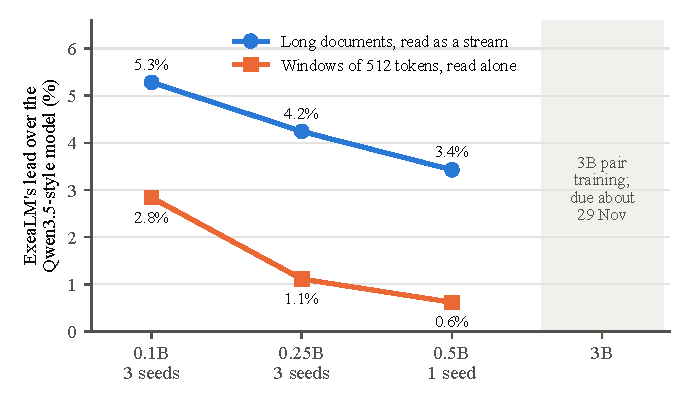
\includegraphics[width=0.58\linewidth]{figs/lead_by_size.pdf}
\caption{ExeaLM's lead over the Qwen3.5-style model by model size, as a percentage of the Qwen3.5-style model's bits per byte (\sect{9}, \sect{10}, \sect{13}, \sect{15}, \sect{20}). The two lines are long documents read as a stream (4,096 tokens) and 512-token windows read alone. Both leads shrink from 0.1B to 0.5B, the long-document lead less, and the 3B pair is still training.}
\label{fig:size}
\end{figure}

\paragraph{Distillation into the weights (\sect{22}).}
We pretrained the 0.1B ExeaLM with 30\% of its tokens written by Qwen3.5-9B-Base.
It scored worse than the same seed trained normally, 1.1592 against 1.1549 (one seed).
What a larger model knows goes into the library instead, where Table~\ref{tab:library} shows a gain.

\paragraph{Agents sharing a board (\sect{14}).}
Three 0.1B ExeaLM agents shared a message board while each read one window of a document.
They scored 1.181, against 1.096 for one 0.1B model reading the same windows as a stream (one seed).
The board itself gained 0.0035 over the same agents with the board cut.
The board is not part of the 9B plan.

\paragraph{ExeaLM's own retrieval circuit (\sect{7}).}
A retrieval circuit inside the model found the right entry for 0.1\% of questions, and attaching the library changed nothing.
The library reaches the model through an ordinary search instead, as in Table~\ref{tab:library}.

%======================================================================== 4
\section{The plan and the ask}

\subsection{The 9B run}

\begin{table}[H]
\centering\small
\caption{The 9B pretraining run. The model and its speed are measured, and the data plan for 1T tokens is still open (\sect{16}, \texttt{docs/budget.md}, \texttt{docs/decisions.md}, \texttt{experiments/recipe/exealm\_recipe\_v2.json}).}
\label{tab:ninebrun}
\begin{tabularx}{\linewidth}{@{}l L@{}}
\toprule
Model & 9,276.8M parameters, 42 layers of width 4,096; attention with gate, QK-norm, value residual and XSA; one TONN layer at layer 21 \\
Data & 1T tokens from data recipe v2.1: research code first, then general code, research papers, math, web text and Japanese. The recipe targets 300B tokens and already repeats Stack Exchange twice, so 1T needs about 3.3 passes on average or a larger build. \\
Recipe & as in the study: the mixed stream phase in the last 20\%, the anneal mix in the last 10\% \\
Compute & about 78,000 H100 GPU-hours: 75,000 at the measured one-node speed, plus about 3,000 for the stream phase \\
Time & about 25 days on 128 H100s (our planning assumption), if the per-GPU speed holds at that scale \\
Code still to write & splitting the weights across GPUs in the training script, as the speed test does, and averaging the TONN layer's running output sizes across GPUs \\
\bottomrule
\end{tabularx}
\end{table}

The 9B run's 108 tokens per parameter are close to the long 0.1B pair's 110, which tests whether ExeaLM's lead holds with long training.

\subsection{Post-training for research and code}

The post-training plan (\texttt{docs/post\_training.md}, a dated draft) has five stages after pretraining (Table~\ref{tab:post}).
Each stage is tested first at 0.5B or 3B, with a control, inside the NAIRR allocation, for about 191 GPU-hours plus about 140 for library v2.
The plan lists the code still to be written for each stage.

\begin{table}[H]
\centering\small
\caption{Post-training stages at 9B (\texttt{docs/post\_training.md}, sections 2.1 to 2.6). These are draft estimates, and together they are about a tenth of pretraining.}
\label{tab:post}
\begin{tabularx}{\linewidth}{@{}l L l r@{}}
\toprule
Stage & What it teaches & Size at 9B & GPU-hours \\
\midrule
A. Long context & papers and code longer than today's 1,024 tokens of exact attention & about 30B tokens & about 2,700 \\
B. Library mid-training & read searched entries and ignore wrong ones & about 15B tokens & about 1,100 \\
C. Supervised fine-tuning & answer research and code requests with entries given & about 2.4M conversations & about 600 \\
D. Reinforcement learning & pass unit tests and reach exact answers & about 60,000 tasks & 500 to 1,000 \\
E. Retrieval as a tool & write its own search queries & inside C and D & \\
Evaluation & & & about 300 \\
Teacher data & DeepSeek-V4-Flash writes library entries and tasks, conversations, code problems with tests and search examples & about 4.9B tokens & about 2,700 \\
\bottomrule
\end{tabularx}
\end{table}

Training and evaluation come to about 5,500 GPU-hours, and the teacher data to about 2,700.

\subsection{The library ships with the model}

The plan in \texttt{docs/library.md} is one repository with the weights, the library text with each passage's source and license, and the search index.
The shipped library holds only text that can be redistributed: the written tier and the 18.8B public tokens of the human tier, published on 27 November with a license and URL on every passage. Left out are arXiv papers under arXiv's default license (5.2B tokens) and Stack Exchange (1.0B), whose license needs each post's author.
A core edition of about 10 GB fits a laptop, and the full edition holds the 25B-token human tier.
The planned interface is one call that loads the model and its library, and one that searches both tiers and answers.
In the planned hosted service, one GPU holds the merged index and serves every copy of the 9B behind a router; at 2.0 ms a query, search adds a few percent to the 9B's 50 to 100 ms of reading a prompt.

\subsection{Memory layers, the next research bet}

Memory layers are large key-value tables that a model reads sparsely, a few entries for each token.
In the abstract of Berges et al.\ (ICML 2025), models with memory layers of up to 128B parameters beat dense models with twice the compute, most of all on factual tasks.
We will test memory layers at 0.1B against the same model with library search (\texttt{docs/library.md}, ``Later'').
They are not part of the funded 9B run.

\subsection{Funding tiers}

Table~\ref{tab:tiers} prices two tiers at the prices of Section~2.6.
The reserve is 30\%, the low end of the 30 to 50\% that \texttt{docs/budget.md} adds to rented runs for restarts, evaluation and data loading.
The study itself lost about 190 of its 2,000 GPU-hours, about 10\%, to one bug.

\begin{table}[H]
\centering\small
\caption{Funding tiers in H100 GPU-hours, with dollars at \$2.69 and \$3.99 per GPU-hour. Pretraining is most of either tier. Serving the 9B model itself to users is not priced here.}
\label{tab:tiers}
\begin{tabularx}{\linewidth}{@{}L r r@{}}
\toprule
Item & Tier 1: train the 9B & Tier 2: Tier 1 and service \\
\midrule
Pretraining on 1T tokens, with the stream phase (Section 2.6) & 78,000 & 78,000 \\
Post-training and evaluation (Table~\ref{tab:post}) & 5,500 & 5,500 \\
Teacher data from DeepSeek-V4-Flash (Table~\ref{tab:post}) & 2,700 & 2,700 \\
Reserve, 30\% & 25,860 & 25,860 \\
Library search service on one H100 for a year (8,760 hours) & none & 8,760 \\
\midrule
\textbf{H100 GPU-hours} & \textbf{112,060} & \textbf{120,820} \\
Dollars at \$2.69 & \$301,000 & \$325,000 \\
Dollars at \$3.99 & \$447,000 & \$482,000 \\
Team support & none & \pend{amount set by the lead} \\
\bottomrule
\end{tabularx}
\end{table}

Tier~1 buys the 9B base and post-trained models, library v2, the evaluation and the open release.
Tier~2 adds a public search service for the library and paid time for the team.

\subsection{Milestones}

\begin{table}[H]
\centering\small
\caption{Milestones. Dated rows come from the repository, and the funded rows count months from the start of funding.}
\label{tab:milestones}
\begin{tabularx}{\linewidth}{@{}l L l@{}}
\toprule
When & Milestone & Paid by \\
\midrule
27 November 2026 & Library v2 research entries due; code entries and tasks follow & NAIRR \\
29 November 2026 & 3B pair finishes in the evening; its scores and benchmarks fill Table~\ref{tab:main} & NAIRR \\
28 November 2026 & The 0.5B run at 20 tokens per parameter finishes (ExeaLM, its attention-only control, the Qwen3.5-style model) & NAIRR \\
Next, in the allocation & Library v2 post-training at 0.5B and 3B for both models; a scaling fit and 9B projection; the small post-training tests & NAIRR \\
Month 1 & The 1T-token data build; weight splitting in the training code; a speed test at full cluster size & Tier 1 \\
Months 2 and 3 & Pretraining, about 25 days on 128 H100s & Tier 1 \\
Month 4 & Post-training stages A to E & Tier 1 \\
Month 5 & Scores on the frozen suite, with and without the library; open release & Tier 1 \\
\bottomrule
\end{tabularx}
\end{table}

\subsection{Risks and what we do about them}

\begin{table}[H]
\centering\small
\caption{Risks to the 9B claim and our response to each. The first two are the largest.}
\label{tab:risks}
\begin{tabularx}{\linewidth}{@{}>{\raggedright\arraybackslash}p{0.33\linewidth} L@{}}
\toprule
Risk & Response \\
\midrule
The 9B trains on far fewer tokens than Qwen3.5-9B (\sect{18}, \texttt{docs/post\_training.md}). With no library, Qwen3.5-9B-Base is far ahead of our 0.25B model (0.674 against 1.011, seed 0). &
The claim is the system with its library. Every benchmark is reported with and without the library, side by side. Every baseline gets the same library and search. Passages that share a 13-token window with any of 14 benchmarks are never given (10 of v1's 18,545 entries). Results with the library are claimed only on benchmarks checked this way. \\
The lead on windows alone shrinks with size and with training length: 0.6\% at 0.5B, and 0.6\% at 0.1B trained to 110 tokens per parameter (2 seeds). &
The long-document lead holds better (4.7\% on the long pair), and the mixed stream phase kept the long pair's second seed 0.008 ahead on windows alone. The 3B result, the 0.5B run at 20 tokens per parameter and a scaling fit all come before any 9B run. \\
ExeaLM's edge in using the library is measured only at 0.1B. &
The library v2 test at 0.5B and 3B, both models with the same recipe. If the edge fades, the library still helps any model and ships as an open data set. \\
The library's questions come from the model that wrote its entries, which suits retrieval. &
External benchmarks (QASPER, BigCodeBench, DS-1000), and a new test on held-out documents that no entry was written from. \\
A 9B trained on the full recipe will have read much of the human tier, which is the recipe's text outside the study's slice. &
The library test for the 9B uses held-out documents and questions no entry was written from, with and without the human tier. \\
Speed across many nodes is timed only up to 4 nodes (16 GPUs). &
At 4 nodes, with the weights split within each node and copied across nodes, the 9B ran at 228 effective TFLOP/s per GPU at 32 rows per GPU (Appendix~C). Month 1 times the full cluster. \\
Some library sources have open license questions (a KAKEN mirror, per-paper licenses of arXiv and peS2o papers, Stack Exchange attribution). &
Only redistributable text is published. These questions are settled before the human tier is published, and a script already separates the part without them. \\
This is the team's first multi-node, multi-week training run. &
The study's record: correctness checked against the CPU, exact resume from checkpoints, and a bug fixed with a test that fails on the old code. The tiers carry a 30\% reserve. \\
\bottomrule
\end{tabularx}
\end{table}

\subsection{The team}

Avneh Bhatia leads ExeaLM and wrote its model, training and evaluation code.
Joshua Selvaraj maintains the code base with him, and the NAIRR proposal names Devom Brahmbhatt as the third team member.
Contributors with merged work include Aaron Chu, Jasraj Tulsi and Eknoor Ahluwalia.
The code has more than 300 automated tests, and the study's decisions are dated in \texttt{docs/decisions.md}.

%======================================================================== 5
\section{Open science}

The code, results, trained models and data behind this report are public, and Appendix~A gives the file behind each number.
The study's finished models are released under Apache-2.0, weights only.

\begin{itemize}
\item Code, results and decisions: \url{https://github.com/exea-labs/ExeaLM/tree/nairr}
\item The study's models: \url{https://huggingface.co/exea-labs/exealm-nairr}
\item Library v1: \url{https://huggingface.co/datasets/exea-labs/exealm-library}
\item Pretraining data (\texttt{slice-30b-r2}): \url{https://huggingface.co/datasets/exea-labs/exealm-pretrain}
\item Post-training data: \url{https://huggingface.co/datasets/exea-labs/exealm-post}
\item Lab notes: \url{https://blog.exealabs.org}
\end{itemize}

For the 9B we plan to release the weights, the code, the training data and the training logs, and the library where its sources' licenses allow.

%======================================================================== appendix
\newpage
\appendix
\section*{Appendix A. Where each number comes from}
\addcontentsline{toc}{section}{Appendix A}

``\sect{N}'' is section N of \texttt{results/expanse/README.md} on branch \texttt{nairr}.
A percentage lead is (Qwen3.5-style minus ExeaLM) divided by Qwen3.5-style, from the bits per byte given.
The figures are drawn by \texttt{docs/funding\_report/figs/}\allowbreak\texttt{make\_figs.py} from the JSON files named.

\begin{table}[H]
\centering\footnotesize
\begin{tabularx}{\linewidth}{@{}L >{\raggedright\arraybackslash}p{0.44\linewidth}@{}}
\toprule
Number & Source \\
\midrule
54 of 54 pairs; windows alone at 0.1B (1.157, 1.190, 1.200); per-pair range 0.024 to 0.061 & \sect{9}, \texttt{text\_100m.json} \\
Long documents at 0.1B (1.096, 1.157); without streams 1.132, lead 0.025 & \sect{10}, \texttt{stream8\_100m.json} \\
0.25B windows alone (1.014, 1.026, 1.041; range 0.007 to 0.026) and long documents (0.955, 0.997) & \sect{13}, \sect{15}, \texttt{text\_250m.json}, \texttt{stream8\_250m.json} \\
0.5B, 2 seeds (0.933, 0.939, 0.958; 0.873, 0.906; 3.6\%; 36 of 36 pairs); seed 0's in-run lead 0.011 to 0.004 & \sect{20}, \texttt{text\_500m\_all.json}, \texttt{stream8\_500m\_all.json} \\
0.5B benchmarks, 2 seeds (0.429, 0.421, 0.417; SciQ 0.032, LAMBADA 0.020) & \sect{20}, \texttt{bench\_<model>\_500m\_4.1x\_s0.json} and \texttt{\_s1.json} \\
3B in-run check at step 14,500 (0.806, 0.813, 0.007); 0.016 at step 7,500, 0.034 at step 3,000; finish on the evening of 29 November & \sect{23} \\
Long pair, 2 seeds: step multiplier 1.18, 1.21 at step 5,000 and 1.34, 1.41 at step 20,000; finals 0.958, 0.963 and 0.902, 0.946; in-run leads 0.009 to 0.001 (seed 0) and 0.006 to 0.008 (seed 1) & \sect{24}, \texttt{text\_111x.json}, \texttt{stream8\_111x.json} \\
Switch at step 31,788; second seed mixed from 28,400 & \texttt{docs/decisions.md}, 26 November (7 p.m.) \\
Attention-only control at 110 tokens per parameter, finished (0.958, 0.960; 0.898, 0.902; 0.944 for the Qwen3.5-style model) & \sect{24}, \texttt{text\_strong\_111x.json}, \texttt{stream8\_strong\_111x.json} \\
0.5B run at 20 tokens per parameter & \texttt{docs/decisions.md}, 27 November (1:45 a.m.) \\
Long pair tokens (10.4B) and tokens per parameter (109.6, 108.9) & \texttt{docs/budget.md}, ``The runs'' \\
16,384 tokens (1.0726, 1.1339, 0.9471, 0.9956; 5.4\%, 4.9\%; 0.043 to 0.048) & \sect{19}, \texttt{stream32\_100m.json} \\
Library v1 (1.645, 0.590, 0.405; 1.633, 0.704, 0.529; 64\%, 21\%, 19\%; 0.110 to 0.116) & \sect{11}, \texttt{library\_rag\_100m\_s0.jsonl} to \texttt{\_s2} \\
BM25 first hit 86.2\% & \sect{8} \\
Qwen3.5-9B-Base (1.031, 0.313, 0.169; 0.674 against 1.011, seed 0) & \sect{18}, \texttt{external\_qwen35\_9b\_base.json} \\
Library v2 tiers and shares (44\%, 28\%, 21\%, 4\%, 2\%), two-tier search (0.44, 0.74, 0.72), search time, index size, prompt-reading estimate; memory layers & \texttt{docs/library.md} \\
DeepSeek-V4-Flash, 13B used per token & \texttt{docs/post\_training.md}, section 3.1 \\
9B speed (206, 40 of 80 GB), 75,000 GPU-hours & \sect{16}, \texttt{nine\_b.json} \\
Stream phase at 1.2 times the cost & \sect{2} \\
All rows of Appendix C & \texttt{nine\_b.json} \\
H100 prices \$2.69 and \$3.99; reserve of 30 to 50\% & \texttt{docs/budget.md}, ``What it costs to rent'' \\
Multi-GPU bug, about 190 GPU-hours & \sect{17} \\
TONN layer against attention: 1.1566, 1.1574 & \sect{19}, \texttt{text\_100m\_strong.json} \\
\phantom{TONN layer against attention: }1.0955, 1.0968 and 1.0726, 1.0737 & \sect{19}, \texttt{stream8\_100m\_strong.json}, \texttt{stream32\_100m.json} \\
\phantom{TONN layer against attention: }long run 1.0316, 1.0348 & \sect{19} \\
Lead by size 0.034, 0.011, 0.006; stream-phase cost 0.007 & \sect{9}, \sect{13}, \sect{20}, \sect{21} \\
Mixed stream phase (1.1532, 1.1546, 1.1496, 1.0969, 1.2085) & \sect{21}, \texttt{text\_mix20distill.json}, \texttt{text\_mix100m.json}, \texttt{docs/decisions.md} \\
Distillation (1.1592, 1.1549) & \sect{22}, \texttt{text\_mix20distill.json} \\
Board (1.181, 1.096, 0.0035); retrieval circuit 0.1\% & \sect{14}, \sect{7} \\
Post-training stages and GPU-hours; 191 and 140 & \texttt{docs/post\_training.md}, sections 2.6 and 5.3 \\
Recipe v2.1 at 300B, Stack Exchange twice & \texttt{experiments/recipe/exealm\_recipe\_v2.json} \\
Rules for results with the library (13-token window, 14 benchmarks, 10 entries) & \texttt{docs/decisions.md}, 26 November (midnight) \\
Paper and code lengths; comparison list; candidate suite & \texttt{docs/post\_training.md}, sections 2.1, 4.2, 4.4, 4.5 \\
Team & NAIRR proposal, section D; \texttt{CONTRIBUTORS.md} \\
\bottomrule
\end{tabularx}
\end{table}

The Appendix~C rows beyond the three in \sect{16} are in \texttt{nine\_b.json} and not yet written up on the results page.
Numbers from \texttt{docs/} are plans and estimates, and the report labels them as such.

\section*{Appendix B. The study's models and runs}
\addcontentsline{toc}{section}{Appendix B}

\begin{table}[H]
\centering\footnotesize
\caption{The three designs (\texttt{docs/budget.md}, \texttt{docs/decisions.md}). All use the same 32k tokenizer, RMSNorm, a SwiGLU MLP and rotary positions. They differ in the non-attention layers and in what the attention layers carry.}
\begin{tabularx}{\linewidth}{@{}l L L L@{}}
\toprule
& ExeaLM & Qwen3.5-style & Plain Llama \\
\midrule
Attention layers & all but the middle layer, with gate, QK-norm, value residual and XSA & 1 of every 4, with gate and QK-norm & every layer, none of the four changes \\
Other layers & one TONN layer at the middle layer & Gated DeltaNet in 3 of every 4 & none \\
Training rows & one window, then streams of four windows in the last 20\% & one window throughout & one window throughout \\
Parameters at 0.1B, 0.25B, 0.5B, 3B & 95.1M, 250.5M, 508.5M, 2,973.5M & 95.7M, 252.1M, 511.3M, 2,986.2M & 89.7M, 234.8M, 474.1M, not trained \\
\bottomrule
\end{tabularx}
\end{table}

\begin{table}[H]
\centering\footnotesize
\caption{Training length per size, the same steps and tokens for every design. A step is 262,144 tokens. Tokens per parameter are ExeaLM's; the smaller plain Llama reads 4.3.}
\begin{tabularx}{\linewidth}{@{}l r r r L@{}}
\toprule
Size & Steps & Tokens & Per parameter & Seeds \\
\midrule
0.1B & 1,468 & 0.4B & 4.0 & 3 \\
0.25B & 3,869 & 1.0B & 4.0 & 3 \\
0.5B & 7,825 & 2.1B & 4.0 & 1 finished, 1 training \\
3B & 45,688 & 12.0B & 4.0 & 1, training \\
0.1B, long pair & 39,735 & 10.4B & 109.6 & 2, training \\
\bottomrule
\end{tabularx}
\end{table}

\section*{Appendix C. The 9B speed rows}
\addcontentsline{toc}{section}{Appendix C}

Rows from \texttt{nine\_b.json}: the full training step of the 9B ExeaLM, 512-token rows, bf16, activation checkpointing, 10 timed steps after 3 warm-up steps.
Only the one-node rows at 2 to 8 rows per GPU are written up (\sect{16}).
``Full'' splits the weights across all GPUs.
``Hybrid'' splits them within each node and copies them across nodes.
Across nodes the speed per GPU depends on the batch.
At 8 rows per GPU, two and four nodes ran at 52 to 103 effective TFLOP/s.
At 228 effective TFLOP/s per GPU (four nodes, 32 rows, hybrid), 1T tokens would take about 68,000 GPU-hours.
The price in this report uses 206, the written-up figure.

\begin{table}[H]
\centering\footnotesize
\begin{tabular}{@{}c c l c r r r@{}}
\toprule
Nodes & GPUs & Sharding & Rows per GPU & Tokens/s per GPU & Effective TFLOP/s per GPU & Peak memory (GB) \\
\midrule
1 & 4 & full & 2 & 2,053 & 114 & 36.8 \\
1 & 4 & full & 4 & 2,938 & 164 & 37.8 \\
1 & 4 & full & 8 & 3,705 & \textbf{206} & 39.8 \\
1 & 4 & full & 16 & 4,183 & 233 & 44.0 \\
1 & 4 & full & 32 & 4,444 & 247 & 52.3 \\
2 & 8 & full & 8 & 1,012 & 56 & 22.5 \\
2 & 8 & full & 16 & 1,949 & 108 & 26.7 \\
2 & 8 & full & 32 & 3,453 & 192 & 35.0 \\
2 & 8 & hybrid & 8 & 1,852 & 103 & 39.8 \\
2 & 8 & hybrid & 16 & 3,290 & 183 & 44.0 \\
2 & 8 & hybrid & 32 & 4,187 & 233 & 52.3 \\
4 & 16 & full & 8 & 928 & 52 & 13.9 \\
4 & 16 & full & 16 & 1,827 & 102 & 18.0 \\
4 & 16 & full & 32 & 3,425 & 191 & 26.3 \\
4 & 16 & hybrid & 8 & 1,359 & 76 & 39.8 \\
4 & 16 & hybrid & 16 & 2,463 & 137 & 44.0 \\
4 & 16 & hybrid & 32 & 4,101 & 228 & 52.3 \\
\bottomrule
\end{tabular}
\end{table}

\end{document}
